% pdflatex -shell-escape software-analysis-main.tex
\documentclass[12pt,openany]{book}

\usepackage{kotex}
\usepackage{commath}
\usepackage{wasysym}
\usepackage{pifont} %http://ctan.org/pkg/pifont\usepackage{slantsc}
\usepackage{hyperref}
\usepackage{stmaryrd} %llbracket
\usepackage{adjustbox}
\usepackage{enumerate}

\usepackage{cite}
\usepackage[numbers]{natbib}
\usepackage{amsthm}

% Define custom theorem styles
\newtheoremstyle{dotless} % Name of the style
{3pt} % Space above
{3pt} % Space below
{\itshape} % Body font
{} % Indent amount
{\bfseries} % Theorem head font
{} % Punctuation after theorem head
{2.5mm} % Space after theorem head
{} % Theorem head spec

\newtheoremstyle{definitionstyle} % Name of the style
{3pt} % Space above
{3pt} % Space below
{} % Body font
{} % Indent amount
{\bfseries} % Theorem head font
{.} % Punctuation after theorem head
{2.5mm} % Space after theorem head
{} % Theorem head spec

% Applying custom styles
\theoremstyle{dotless}
\newtheorem{proposition}{Proposition}[section] % Theorem environment with section-wise numbering
\newtheorem{theorem}{Theorem}[section] % Theorem environment with section-wise numbering
\newtheorem{lemma}[theorem]{Lemma} % Lemma shares the counter with theorem
\newtheorem{corollary}[theorem]{Corollary} % Corollary shares the counter with theorem

\theoremstyle{definitionstyle}
\newtheorem*{observation}{\textcolor{Magenta}{Observation}}
\newtheorem{definition}{Definition}[section] % Definition shares the counter with theorem
\newtheorem{example}{Example}[section] % Example shares the counter with theorem
\newtheorem{exercise}{Exercise}[section] % Example shares the counter with theorem
\newtheorem{remark}{Remark}[section] % Remark shares the counter with theorem
\newtheorem*{note}{Note}

\input{preamble/layout}
\input{preamble/tcolorbox}
\usepackage{tikz}
\usepackage{tikz-cd}
\usetikzlibrary{arrows, positioning}
\usetikzlibrary{shadows}
\usetikzlibrary{shapes.geometric, arrows.meta, positioning}
\input{preamble/algorithm}
\input{preamble/listing}
\newcommand{\A}{\mathbb{A}}
\newcommand{\B}{\mathbb{B}}
\newcommand{\C}{\mathbb{C}}
\newcommand{\F}{\mathbb{F}}
\newcommand{\N}{\mathbb{N}}
\newcommand{\Q}{\mathbb{Q}}
\newcommand{\R}{\mathbb{R}}
\newcommand{\Z}{\mathbb{Z}}

\newcommand{\cP}{\mathcal{P}}
\newcommand{\cR}{\mathcal{R}}

\newcommand{\pl}{\textsf{PL}\ }
\newcommand{\fol}{\textsf{FOL}\ }
\newcommand{\hol}{\textsf{HOL}\ }

\newcommand{\oracle}{\textsc{Oracle}}
\newcommand{\sub}[1]{\textsf{sub}\left(#1\right)}

\newcommand{\dom}{\mathsf{dom}}
\newcommand{\cdm}{\mathsf{cdm}}
\newcommand{\range}{\mathsf{range}}

\newcommand{\free}{\mathsf{free}}
\newcommand{\bound}{\mathsf{bound}}

\newcommand{\true}{\textcolor{red}{\texttt 1}}
\newcommand{\false}{\textcolor{red}{\texttt 0}}
\newcommand{\id}{\textnormal{id}}

\newcommand{\sol}{\textcolor{magenta}{\bf Sol}}
\newcommand{\ie}{i.\,e.}
\newcommand{\eg}{e.\,g.}
\newcommand{\wrt}{w.\,r.\,t.\ }
\newcommand{\aka}{a.\,k.\,a.\ }
\newcommand{\cf}{cf.\ }
\newcommand{\etc}{etc.\ }

\newcommand{\coa}{\mathsf{COA}}
\newcommand{\kpa}{\mathsf{KPA}}
\newcommand{\cpa}{\mathsf{CPA}}
\newcommand{\cca}{\mathsf{CCA}}
\newcommand{\acca}{\mathsf{CCA2}}

\newcommand{\EasyCrypt}{\textsc{EasyCrypt}\ }\usetikzlibrary{arrows, positioning}

\begin{document}
	
	\begin{titlepage}
    \centering
    
    \vspace*{1cm}
    
    \Huge\textsf{\textbf{EasyCrypt - CodeCraftLab}}
    
    \vspace{0.5cm}
%   \LARGE\textsf{- A Deep Dive into Testing and Validation -}
    \LARGE\textsf{- Mastering the Art of EasyCrypt Programming -}
    
    \vspace{1.5cm}
    \textbf{Ji, Yong-Hyeon}

	\vspace{2cm}
%	\begin{figure}[h!]\centering
%	\begin{tikzpicture}
%		% Set colors for different logics
%		\definecolor{plcolor}{RGB}{255, 204, 204}
%		\definecolor{folcolor}{RGB}{204, 229, 255}
%		\definecolor{holcolor}{RGB}{204, 255, 204}
%		
%		% Draw the Higher-Order Logic (HOL) circle
%		\fill[holcolor] (0,0) circle (6cm);
%		\draw (0,0) circle (6cm);
%		\node at (0, 5.25) {\bf Higher-Order Logic (HOL)};
%		
%		% Draw the First-Order Logic (FOL) circle
%		\fill[folcolor] (0,0) circle (5cm);
%		\draw (0,0) circle (5cm);
%		\node at (0, 3.75) {\bf First-Order Logic (FOL)};
%		
%		% Draw the Propositional Logic (PL) circle
%		\fill[plcolor] (0,0) circle (3cm);
%		\draw (0,0) circle (3cm);
%		\node at (0, 0) {\bf Propositional Logic (PL)};
%		
%	\end{tikzpicture}
%	\end{figure}
%	\begin{center}
%	\adjustbox{scale=.9}{
%	\begin{tikzpicture}
%		
%		% Define colors
%		\definecolor{plcolor}{RGB}{255, 153, 153}
%		\definecolor{folcolor}{RGB}{153, 204, 255}
%		\definecolor{holcolor}{RGB}{153, 255, 153}
%		
%		% Draw the Higher-Order Logic (HOL) ellipse
%		\fill[holcolor, draw=black] (0,0) ellipse (8cm and 5cm);
%		\node at (0, 4.4) {\textbf{Higher-Order Logic (HOL)}};
%		
%		% Draw the First-Order Logic (FOL) ellipse
%		\fill[folcolor, draw=black] (0,0) ellipse (6cm and 4cm);
%		\node at (0, 3.4) {\textbf{First-Order Logic (FOL)}};
%		
%		% Draw the Propositional Logic (PL) ellipse
%		\fill[plcolor=, draw=black] (0,0) ellipse (4cm and 3cm);
%		\node at (0, 2.4) {\textbf{Propositional Logic (PL)}};
%		
%		% Add arrows to show inclusion
%%		\draw[thick,-Stealth] (0,0) -- (.5,-1.25) node[midway,above] {\footnotesize More expressive};
%%		\draw[thick,->] (2,1.2) -- (2.7,1.5);
%%		\draw[thick,->] (1.5,-1.2) -- (2.3,-1.5);
%		
%		% Add dimensions
%		\node at (1,-2.5) {\textbullet \, HOL: Functions, Predicates, Quantifiers};
%		\node at (.5,-1.25) {\textbullet \, FOL: Predicates, Quantifiers};
%		\node at (0,0) {\textbullet \, PL: Propositions};
%	\end{tikzpicture}}
%\end{center}
	
	\vspace{1.5cm}
    \vfill
    A document presented for the EasyCrypt
    
    \vspace{0.8cm}
    {\bf\large\textsf{Department of Information Security, Cryptology, and Mathematics}\par}
    {\large\textsf{College of Science and Technology}\par}
    {\large\textsf{Kookmin University}\par}
    \vspace{.25in}
    {\large \textsf{\today}\par}
    
%    \Large{Institution Name}\\
%    Date
\end{titlepage}


	\tableofcontents
	\newpage
	\section*{Symbols}
In this paper, symbols are defined as follows. \\ \ \\ 
$
\begin{array}{cl}
	I\models P & \text{$I$ satisfies $P$} \\
	I\not\models P & \text{$I$ does not satisfies $P$} \\
\end{array}
$
	
	\newpage
	\chapter{Mathematical Background}
	\textbf{Lemma} \\[5pt]
For any boolean values \( a \) and \( b \):
\[
\neg (a \lor b) \Leftrightarrow (\neg a \land \neg b)
\]

\textbf{Proof.} \\[5pt]
We need to show both directions of the equivalence:
\[
\neg (a \lor b) \Rightarrow (\neg a \land \neg b) \quad \text{and} \quad (\neg a \land \neg b) \Rightarrow \neg (a \lor b)
\]

\textbf{First Direction:} \( \neg (a \lor b) \Rightarrow (\neg a \land \neg b) \)

1. Assume \( \neg (a \lor b) \).

2. To show \( \neg a \):
\begin{itemize}
	\item \textbf{Case} \( a = \text{true} \):
	\[
	a = \text{true} \Rightarrow a \lor b = \text{true} \Rightarrow \text{contradiction with } \neg (a \lor b).
	\]
	\item Therefore, \( \neg a \).
\end{itemize}

3. To show \( \neg b \):
\begin{itemize}
	\item \textbf{Case} \( b = \text{true} \):
	\[
	b = \text{true} \Rightarrow a \lor b = \text{true} \Rightarrow \text{contradiction with } \neg (a \lor b).
	\]
	\item Therefore, \( \neg b \).
\end{itemize}

4. We conclude that \( \neg (a \lor b) \Rightarrow (\neg a \land \neg b) \).

\textbf{Second Direction:} \( (\neg a \land \neg b) \Rightarrow \neg (a \lor b) \)

1. Assume \( \neg a \land \neg b \).

2. Consider \( a \lor b \):
\begin{itemize}
	\item \textbf{Case} \( a = \text{true} \): Contradicts \( \neg a \).
	\item \textbf{Case} \( b = \text{true} \): Contradicts \( \neg b \).
\end{itemize}

3. Therefore, \( (\neg a \land \neg b) \Rightarrow \neg (a \lor b) \).

\textbf{Conclusion:}
\[
\neg (a \lor b) \Leftrightarrow (\neg a \land \neg b)
\]

textbf{Lemma} \\[5pt]
For any boolean values \( a \) and \( b \):
\[
\neg (a \lor b) \Leftrightarrow (\neg a \land \neg b)
\]

\textbf{Proof.} \\[5pt]
\begin{align*}
	&\text{1. To prove:} \quad \neg (a \lor b) \Rightarrow (\neg a \land \neg b) \\
	&\quad \text{Assume:} \quad \neg (a \lor b) \\
	&\quad \text{Then, we have:} \\
	&\quad a = \text{true} \Rightarrow a \lor b = \text{true} \Rightarrow \bot \Rightarrow \neg a \\
	&\quad b = \text{true} \Rightarrow a \lor b = \text{true} \Rightarrow \bot \Rightarrow \neg b \\
	&\quad \therefore \neg a \land \neg b \\
	\\
	&\text{2. To prove:} \quad (\neg a \land \neg b) \Rightarrow \neg (a \lor b) \\
	&\quad \text{Assume:} \quad \neg a \land \neg b \\
	&\quad \text{Then,} \quad a \lor b = \text{true} \Rightarrow a = \text{true} \lor b = \text{true} \Rightarrow \bot \\
	&\quad \therefore \neg (a \lor b) \\
	\\
	&\text{Conclusion:} \quad \neg (a \lor b) \Leftrightarrow (\neg a \land \neg b)
\end{align*}

	
	\newpage
	\chapter{Cryptographic Background}
	\section{Attacker Type}
\begin{itemize}
	\item $\coa$; Ciphertext-Only Attack
	\item $\kpa$; Known-Plaintext Attack
	\item $\cpa$; Chosen-Plaintext Attack
	\item $\cca$; Chosen-Ciphertext Attack
	\item $\acca$; Adaptive Chosen-Ciphertext Attack
\end{itemize}
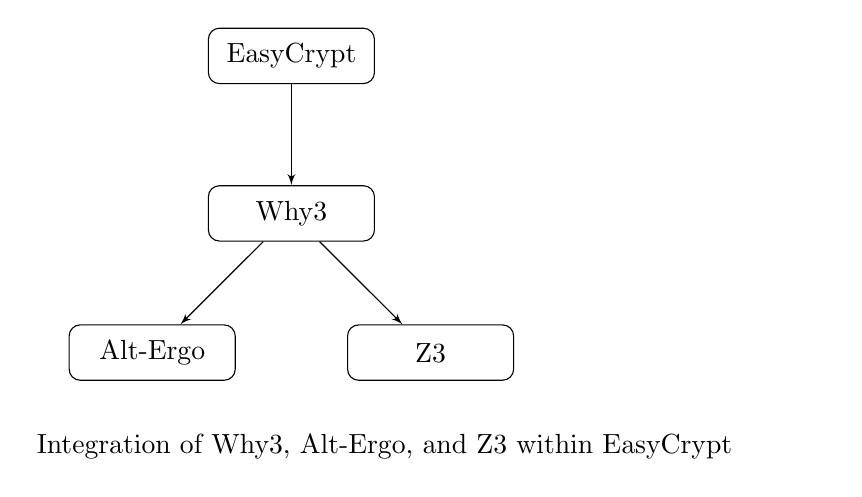
\begin{tikzpicture}[auto, node distance=2cm, >=latex']
	
	% Nodes
	\node [draw, rectangle, rounded corners, text centered, minimum height=2em, minimum width=6em] (easycrypt) {EasyCrypt};
	\node [draw, rectangle, rounded corners, below of=easycrypt, node distance=2cm, text centered, minimum height=2em, minimum width=6em] (why3) {Why3};
	\node [draw, rectangle, rounded corners, below left of=why3, node distance=2.5cm and 1.5cm, text centered, minimum height=2em, minimum width=6em] (altergo) {Alt-Ergo};
	\node [draw, rectangle, rounded corners, below right of=why3, node distance=2.5cm and 1.5cm, text centered, minimum height=2em, minimum width=6em] (z3) {Z3};
	
	% Arrows
	\draw [->] (easycrypt) -- (why3);
	\draw [->] (why3) -- (altergo);
	\draw [->] (why3) -- (z3);
	
	% Labels
	\node [below of=altergo, node distance=1.2cm] (label1) {};
	\node [below of=z3, node distance=1.2cm] (label2) {};
	\node [text width=10cm] at (label1 -| label2) {Integration of Why3, Alt-Ergo, and Z3 within EasyCrypt};
	
\end{tikzpicture}\\


\begin{itemize}
	\item $\mathcal{K}$: key space
	\item $\mathcal{N}$: nonce space
	\item $\mathcal{P}$: plaintext space
	\item $\mathcal{C}$: ciphertext space
\end{itemize}
\[
\texttt{used\_once}(n, \mathcal{N}) = n\in\mathcal{N}.
\]\[
\fullfunction{\texttt{used\_once}}{\mathcal{N}\times\set{\mathcal{N}}}{\set{0,1}}{(n,\mathcal{N})}{n\in\mathcal{N}}\]

\[
\texttt{used\_once}:\mathcal{N}\to[\set{\mathcal{N}}\to\set{0,1}]
\]
%현대 암호학에서는 공격자의 능력치에 따라 공격 유형을 다음과 같이 분류한다.
%1. 암호문 단독 공격()
%− 1개 이상의 암호문이 주어진 상황에서, 각 암호문에 대한 평문을 복원하는 공격
%2. 기지 평문 공격()
%− 동일한 키로 암호화한 평문/암호문 쌍이 1쌍 이상 주어진 상황에서, 동일한 키로 암호화한 새로운 암호문에 대한 평문을
%복원하는 공격
%3. 선택 평문 공격()
%− 공격자가 1개 이상의 원하는 평문에 대한 암호문을 얻은 후, 새롭게 주어진 암호문에 대한 평문을 복원하는 공격
%4. 선택 암호문 공격()12
%− 공격자가 1개 이상의 원하는 암호문에 대한 평문을 얻은 후, 새롭게 주어진 암호문에 대한 평문을 복원하는 공격
	
	\newpage
	\chapter{Installing EasyCrypt}
	\input{chapter/ec-chap3}
		
	\newpage
	\appendix
	\chapter{Boolean Functions}
%	\input{appendix/sv-appendix-A}
	
	\bibliographystyle{plain}
	\bibliography{ec-references}	
\end{document}
